\documentclass[11pt,a4paper,final]{article} %draft

\usepackage[T1,T2A]{fontenc}
\usepackage[utf8]{inputenc}
\usepackage[english, russian]{babel}

\usepackage[final]{pdfpages}

\usepackage{textcomp,enumitem}

\usepackage{amsmath,amsthm,amssymb}

\usepackage{fancyhdr} % для настройки страницы и колонтитулов

\usepackage{graphicx}

\usepackage{indentfirst} % автоматический отступ в начале каждого раздела

\usepackage[unicode, pdftex, colorlinks, urlcolor=blue]{hyperref}

\usepackage[left=2cm,right=2cm,top=2cm,bottom=2cm,bindingo ffset=0cm]{geometry}

\linespread{1.3} % устанавливает междустрочный интервал

\pagestyle{plain} % для отображения номеров внизу 

\usepackage{float}

\usepackage{listings} 

\usepackage{pdflscape}
\usepackage{listings} 
\definecolor{darkgreen}{rgb}{0,0.5,0}

\lstset{
backgroundcolor=\color{white},  % Отключаем стандартный фон
basicstyle=\ttfamily\small\fontfamily{inconsolata}\selectfont,
commentstyle=\color{darkgreen}\slshape,
keywordstyle=\color{blue}\bfseries,
numberstyle=\scriptsize\color{gray},
stringstyle=\color{orange},
breakatwhitespace=false,
breaklines=true,
captionpos=b,
keepspaces=true,
numbers=left,
numbersep=3pt,
showspaces=false,
showstringspaces=false,
showtabs=false,
tabsize=4,
language=c++,
captionpos=b,
xleftmargin=0mm,
frame=single,
framerule=0.25mm,
literate=
{а}{{\selectfont\char224}}1
{б}{{\selectfont\char225}}1
{в}{{\selectfont\char226}}1
{г}{{\selectfont\char227}}1
{д}{{\selectfont\char228}}1
{е}{{\selectfont\char229}}1
{ж}{{\selectfont\char230}}1
{з}{{\selectfont\char231}}1
{и}{{\selectfont\char232}}1
{й}{{\selectfont\char233}}1
{к}{{\selectfont\char234}}1
{л}{{\selectfont\char235}}1
{м}{{\selectfont\char236}}1
{н}{{\selectfont\char237}}1
{о}{{\selectfont\char238}}1
{п}{{\selectfont\char239}}1
{р}{{\selectfont\char240}}1
{с}{{\selectfont\char241}}1
{т}{{\selectfont\char242}}1
{у}{{\selectfont\char243}}1
{ф}{{\selectfont\char244}}1
{х}{{\selectfont\char245}}1
{ц}{{\selectfont\char246}}1
{ч}{{\selectfont\char247}}1
{ш}{{\selectfont\char248}}1
{щ}{{\selectfont\char249}}1
{ъ}{{\selectfont\char250}}1
{ы}{{\selectfont\char251}}1
{ь}{{\selectfont\char252}}1
{э}{{\selectfont\char253}}1
{ю}{{\selectfont\char254}}1
{я}{{\selectfont\char255}}1
{А}{{\selectfont\char192}}1
{Б}{{\selectfont\char193}}1
{В}{{\selectfont\char194}}1
{Г}{{\selectfont\char195}}1
{Д}{{\selectfont\char196}}1
{Е}{{\selectfont\char197}}1
{Ж}{{\selectfont\char198}}1
{З}{{\selectfont\char199}}1
{И}{{\selectfont\char200}}1
{Й}{{\selectfont\char201}}1
{К}{{\selectfont\char202}}1
{Л}{{\selectfont\char203}}1
{М}{{\selectfont\char204}}1
{Н}{{\selectfont\char205}}1
{О}{{\selectfont\char206}}1
{П}{{\selectfont\char207}}1
{Р}{{\selectfont\char208}}1
{С}{{\selectfont\char209}}1
{Т}{{\selectfont\char210}}1
{У}{{\selectfont\char211}}1
{Ф}{{\selectfont\char212}}1
{Х}{{\selectfont\char213}}1
{Ц}{{\selectfont\char214}}1
{Ч}{{\selectfont\char215}}1
{Ш}{{\selectfont\char216}}1
{Щ}{{\selectfont\char217}}1
{Ъ}{{\selectfont\char218}}1
{Ы}{{\selectfont\char219}}1
{Ь}{{\selectfont\char220}}1
{Э}{{\selectfont\char221}}1
{Ю}{{\selectfont\char222}}1
{Я}{{\selectfont\char223}}1,
numbers=left, % пронумеровать строки с левой стороны
breaklines=true % разрешает автоматический перенос строк
}

\hypersetup{
colorlinks=true, % делает ссылки цветными вместо рамки
linkcolor=blue, % цвет внутренних ссылок
urlcolor=blue, % цвет внешних ссылок
citecolor=blue % цвет ссылок на литературу в тексте
}

\textheight=24cm 
\textwidth=16cm
\oddsidemargin=0pt 
\topmargin=-1.5cm
\parindent=24pt 
\parskip=0pt 
\tolerance=2000 
\flushbottom 

%\usepackage[font=scriptsize]{caption}
\usepackage[labelsep=period]{caption}

\usepackage{amsmath}
\usepackage{colortbl} 
\usepackage{multirow} 
\usepackage{tabularx}
\usepackage{arydshln}

\begin{document}

\thispagestyle{empty}

\begin{center}
{\Large МИНОБРНАУКИ РОССИИ}\\
~\\
{\large ФЕДЕРАЛЬНОЕ ГОСУДАРСТВЕННОЕ БЮДЖЕТНОЕ ОБРАЗОВАТЕЛЬНОЕ УЧРЕЖДЕНИЕ ВЫСШЕГО ПРОФЕССИОНАЛЬНОГО ОБРАЗОВАНИЯ}\\
~\\
{\Large \bf <<САНКТ-ПЕТЕРБУРГСКИЙ ПОЛИТЕХНИЧЕСКИЙ УНИВЕРСИТЕТ ПЕТРА ВЕЛИКОГО>>}\\
~\\
{\large Институт компьютерных наук и кибербезопасности }\\
{\large Высшая школа технологий искусственного интеллекта}\\
{\large Направление 02.03.01 Математика и компьютерные науки}\\
~\\
~\\
~\\
~\\
{\Large \bf  Отчет по курсовой работе}\\
\vspace{3mm}
{\Large {по дисциплине <<Теория алгоритмов>>}}\\
\vspace{3mm}
{\Large \bf Синтез функциональной схемы часов }\\
\vspace{3mm}
{\Large Вариант № 21}
~\\
~\\
~\\
~\\
~\\
{\large Обучающийся: \underline{\hspace{3.5cm}} \hspace{12mm} Шихалев А.О.}\\
~\\
{\large Преподаватель: \underline{\hspace{3.5cm}} \hspace{12mm} Востров А.В.}\\
~\\
~\\
~\\
~\\
\end{center}
\begin{flushright}

«\underline{\hspace{1cm}}»\underline{\hspace{3cm}}20\underline{\hspace{0.7cm}}г.
\end{flushright}
~\\
~\\
~\\
\begin{center}
{\large Санкт-Петербург, 2025}
\end{center}

\newpage

\tableofcontents

\newpage
\section* {Введение}
\addcontentsline{toc}{section}{Введение}
Курсовая работа представляет из себя спроектированную схему, реализующую поведение часов со следующими характеристиками:
\begin{itemize}
	\item Отображение и корректировка минут, часов в 12-часовом формате.
	\item Простой секундомер (сброс-запуск-остановка).
	\item Остановка часов по нажатию кнопки.
\end{itemize}
\par Курсовая работа реализована в Logisim 2.7.1.


\newpage
\section{Постановка задачи}
Требуется построить функциональную схему электронных часов в соответствии с вариантом 1001100 (21 Вариант):
\begin{itemize}
	\item Отображение и корректировка минут, часов. 
	\item 12-и часовой формат времени.
	\item Простой секундомер (сброс-запуск-остановка).
	\item Остановка часов по нажатию кнопки.
\end{itemize}
Для построения функциональной схемы часов требуется выполнить следующие 6 этапов:
\begin{enumerate}
	\item Построить граф управляющего автомата часов и дать пояснения к нему. 
	\item Провести кодирование входных и выходных воздействий и состояний автомата.
	\item Построить минимизацию функций блоков F и FL.
	\item Построить общую функциональную схему. При этом необходимо четко описать алгоритм работы и уметь
	объяснить принцип проектирования всех блоков.
	\item Определить (приблизительно) площадь микросхемы, реализующей построенную функциональную схему
	при современной плотности компоновки транзисторов.
\end{enumerate}


\newpage
\section{Математическое описание}
\subsection{Конечный автомат}
Математическая модель дискретного устройства, которая описывается набором $S = (S, X, Z, \delta, \lambda, a_0)$, где 
\begin{itemize}
	\item S = $\{s_0,…, s_m,…, s_M\}$ –- множество состояний;
	\item X = $\{x_1 ,…, x_f ,…, x_F\}$ –- множество входных сигналов;
	\item Z = $\{z_1 ,…, z_g ,…, z_G\}$ -- множество выходных сигналов;
	\item $\Delta$ -- функция переходов КА, которая $(s_m, x_f) \rightarrow s_s$, т.е. $s_s= \delta(s_m,x_f), s_s \in S$.
	\item $\Lambda$ –- функция выходов КА, которая $(s_m, x_f) \rightarrow z_g$, т.е. $z_g= \lambda(s_m,x_f), z_g\in Z$.
	\item $s_0$ –- начальное состояние. 
\end{itemize}
\par Конечный автомат работает в дискретные моменты времени, и в момент времени t=0 автомат всегда находится в состоянии $s_0$.
\par Управление часами несложно задать при помощи конечного автомата Мили.


\subsection{Синтезированный граф конечного автомата для часов}
На \hyperref[fig:graph]{рисунке 1} изображён граф конечного автомата для часов:

\newpage
\begin{figure}[H]
	\centering
	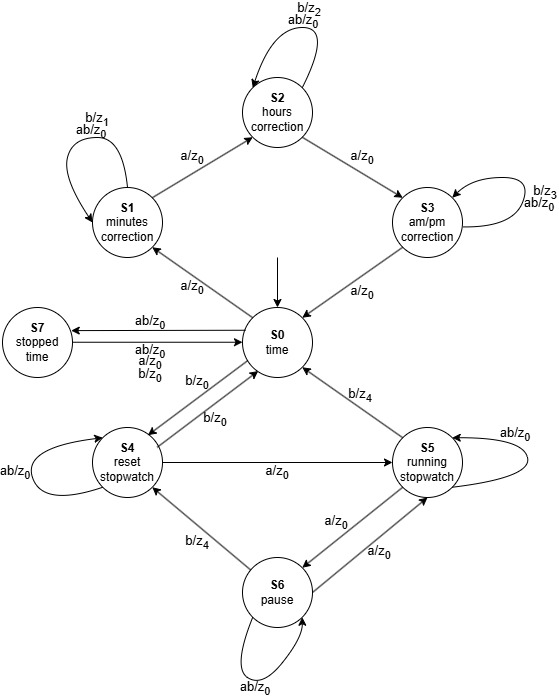
\includegraphics[width=1.00\linewidth]{img/automaton.jpg}
	\caption{Граф конечного автомата для часов}
	\label{fig:graph}
\end{figure}


\subsubsection{Входы конечного автомата}
Входной алфавит конечного автомата состоит из 4-х элементов: по отдельности нажатые кнопки a, b и зажатые вместе кнопки ab. 
\[X = \{a, b, ab\}\]
Входной алфавит можно закодировать следующим образом:
\begin{itemize}[itemsep=0pt]
	\item $a \rightarrow 00$
	\item $b \rightarrow 01$
	\item $ab \rightarrow 10$
	% \item $abc \rightarrow 11$
\end{itemize}


\subsubsection{Состояния конечного автомата}
Описание состояний и переходов управляющего автомата:
\begin{itemize}
	\item[$s_0$] \textbf{time} - состояние отображения текущего времени. На индикаторах значения часов, минут.
	\item[$s_1$] \textbf{minutes correction} - состояние корректировки минут. При переходе в это состояние гаснут индикаторы отображения часов. Однократное нажатие кнопки ''b'' добавляет единицу к значению минут, отображаемому на индикаторе минут.
	\item[$s_2$] \textbf{hours correction} - состояние корректировки часов. Свидетельством того, что часы готовы к корректировке часов, является погасшие индикаторы отображения минут и am/pm. Однократное нажатие кнопки “b” добавляет
	единицу к значению часов.
	\item[$s_3$] \textbf{am/pm correction} -  состояние смены am на pm и наоборот -- производится при нажатии на кнопку ''b''.
	
	\item[$s_4$]\textbf{ reset stopwatch} - состояние остановленного секундомера. На индикаторах - минуты и секунды секундомера, они отображаются вместо часов и минут. В этом состоянии секундомер не отсчитывает время. Нажатием кнопки ''b'' возможно сбросить накопленное отображаемое значение, нажатием кнопки ''a'' - запустить секундомер.
	
	\item[$s_5$] \textbf{running stopwatch} - состояние запущенного секундомера. На индикаторах - идущее время (минуты и секунды) секундомера. Нажатием кнопки ''а'' можно поставить секундомер на паузу (иначе говоря, перевести его в состояние pause). Нажатием кнопки ''b'' часы можно перевести в состояние отображения времени, секундомер при этом сбросится.
	
	\item[$s_6$] \textbf{pause} - состояние поставленного на паузу секундомера. При нажатии на кнопку ''a'' секундомер возобновит свою работу -- перейдет в состояние running stopwatch. В случае нажатия на кнопку ''b'' будет произведен сброс секундомера и переход в состояние reset stopwatch.
	
	\item[$s_7$] \textbf{stopped time} - состояние установки минут будильника. При переходе в это состояние гаснут индикаторы отображения часов и am/pm. Нажатие на любую кнопку вернет часы в исходное состояние time.
\end{itemize}

\par Функция переходов КА представлена в \hyperref[tab:transition]{таблице 1}:

\begin{table}[H]
	\centering
	\begin{tabular}{|>{\cellcolor{cyan!20}}c|c|c|c|}
		\hline
		\rowcolor{cyan!20}
		$\Delta$ & a & b & ab \\ 
		\hline
		$s_0$ & $s_1$ & $s_4$ & $s_7$ \\ 
		\hline
		$s_1$ & $s_2$ & $s_1$ & $s_1$ \\ 
		\hline
		$s_2$ & $s_3$ & $s_2$ & $s_2$ \\ 
		\hline
		$s_3$ & $s_0$ & $s_3$ & $s_3$ \\ 
		\hline
		$s_4$ & $s_5$ & $s_0$ & $s_4$ \\ 
		\hline
		$s_5$ & $s_6$ & $s_0$ & $s_5$ \\ 
		\hline
		$s_6$ & $s_5$ & $s_4$ & $s_6$ \\ 
		\hline
		$s_7$ & $s_0$ & $s_0$ & $s_0$ \\ 
		\hline
	\end{tabular}

\label{tab:transition}
\caption{Таблица функции переходов конечного автомата.}
\end{table}

\par Множество состояний конечного автомата выглядит следующим образом: 
\[S = \{s_0, s_1, s_2, s_3, s_4, s_5, s_6, s_7\}\]
\par Также следует отметить, что начальным состоянием конечного автомата является состояние $s_0$ - time.
\par В \hyperref[tab:stages]{таблице 2} приведены коды необходимых для реализации состояний.

\begin{table}[H]
	\begin{center}
		\begin{tabular}{|c|l|c|}
			\hline
			Состояние & Расшифровка & Код \\ 
			\hline
			{$ s_0 $} & time & 000 \\ 
			{$ s_1 $} & minutes correction & 001 \\ 
			{$ s_2 $} & hours correction & 010 \\
			{$ s_3 $} & am/pm correction & 011 \\
			{$ s_4 $} & reset stopwatch & 100 \\			
			{$ s_5 $} & running stopwatch & 101 \\
			{$ s_6 $} & pause & 110 \\ 
			{$ s_7 $} & stopped time & 111 \\ 
			\hline
		\end{tabular}
	\end{center}
	\caption{Коды состояний}
	\label{tab:stages}
\end{table}

\newpage
\subsubsection{Выходы конечного автомата}
Описание выходов управляющего автомата:

\begin{itemize}[itemsep=-8pt, topsep=-2pt]
	\item $z_0$ - Нейтральный сигнал;
	\item $z_1$ - Корректировка минут;
	\item $z_2$ - Корректировка часов;
	\item $z_3$ - Смена am/pm;
	\item $z_4$ - Сброс секундомера;
\end{itemize}
\par В таком случае множество выходов конечного автомата можно записать следующим образом:
\[Z = \{z_0, z_1, z_2, z_3, z_4\}\]


\par В \hyperref[tab:out]{таблице 3} представлена функция выходов конечного автомата: \\

\begin{table}[H]
	\centering
	% \vspace{10mm} % Adjust the height of the space between caption and tabular
	\begin{tabular}{|>{\cellcolor{cyan!20}}c|c|c|c|c|}
		\hline
		\rowcolor{cyan!20}
		$\Lambda$ & a & b & ab \\ 
		\hline
		$s_0$ & $z_0$ & $z_0$ & $z_0$ \\ 
		\hline
		$s_1$ & $z_0$ & $z_1$ & $z_0$ \\ 
		\hline
		$s_2$ & $z_0$ & $z_2$ & $z_0$ \\ 
		\hline
		$s_3$ & $z_0$ & $z_3$ & $z_0$ \\ 
		\hline
		$s_4$ & $z_0$ & $z_0$ & $z_0$ \\ 
		\hline
		$s_5$ & $z_0$ & $z_4$ & $z_0$ \\ 
		\hline
		$s_6$ & $z_0$ & $z_4$ & $z_0$ \\ 
		\hline
		$s_7$ & $z_0$ & $z_0$ & $z_0$ \\ 
		\hline
	\end{tabular}
	\caption {Таблица функции выходов конечного автомата.}
	\label{tab:out}
\end{table}



\subsection{Управляющие воздействия}

\par Входом в управляющий автомат являются преобразованные внешние воздействия, выходы – это два типа
управляющих воздействий: импульсные и потенциальные. 

\par {\bf Импульсные микрокоманды} -- это кратковременные воздействия, которые подаются в момент нажатия внешних кнопок владельцем часов. Значение импульсной микрокоманды (кратковременное воздействие) может быть отлично от нуля лишь во время перехода из одного состояния в другое. В \hyperref[tab:impulse]{таблице 4} приведены импульсные микрокоманды.

\begin{table}[H]
	\captionsetup{skip=0pt}
\begin{center}
	\begin{tabular}{|c|c|}
		\hline
		Обозначение & Расшифровка \\ 
		\hline
		$ i_1 $ & Добавление единицы в счётчик минут \\
		$ i_2 $ & Добавление единицы в счётчик часов \\
		$ i_3 $ & Смена am/pm \\
		$ i_4 $ & Сброс секундомера \\
		\hline
	\end{tabular}
\end{center}
\caption{Импульсные микрокоманды}
\label{tab:impulse}
\end{table}

\par {\bf Потенциальные микрокоманды} -- это продолжительное воздействие, которое действует в период нахождения автомата в определенном состоянии и может измениться только при переключении автомата в другое состояние. В \hyperref[tab:impulse]{таблице 5} приведены потенциальные микрокоманды.

\begin{table}[H]
	\captionsetup{skip=0pt}
	\begin{center}
		\begin{tabular}{|c|c|}
			\hline
			Обозначение & Расшифровка \\ 
			\hline
			$ L_1 $ & Отображение минут \\
			$ L_2 $ & Отображение часов \\
			$ L_3 $ & Отображение am/pm \\
			$ L_4 $ & Отображение секунд и минут у секундомера \\
			$ L_5 $ & Подключение счетчиков часов к генератору тактовых импульсов \\
			$ L_6 $ & Подключение счетчиков секундомера к генератору тактовых импульсов \\
			\hline
		\end{tabular}
	\end{center}
	\caption{Импульсные микрокоманды}
	\label{tab:impulse}
\end{table}

\subsection{Таблица истинности для преобразования FL}

Связь состояний конечного автомата с потенциальными микрокомандами представлена в \hyperref[tab:FL]{таблице 6}.

\begin{table}[H]
	\centering
	\begin{tabular}{|>{\cellcolor{cyan!20}}c|c|c|c|c|c|c|c|c|c|c|}
		\hline
		\rowcolor{cyan!20}
		$s_i$ & $q_1$ & $q_2$ & $q_3$ & $L_1$ & $L_2$ & $L_3$ & $L_4$ & $L_5$ & $L_6$  \\ 
		\hline
		$s_0$ & 0 & 0 & 0 & 1 & 1 & 1 & 0 & 1 & 0 \\ 
		\hline
		$s_1$ & 0 & 0 & 1 & 1 & 0 & 0 & 0 & 0 & 0 \\ 
		\hline
		$s_2$ & 0 & 1 & 0 & 0 & 1 & 0 & 0 & 0 & 0 \\ 
		\hline
		$s_3$ & 0 & 1 & 1 & 0 & 0 & 1 & 0 & 0 & 0 \\ 
		\hline
		$s_4$ & 1 & 0 & 0 & 0 & 0 & 0 & 1 & 1 & 0 \\ 
		\hline
		$s_5$ & 1 & 0 & 1 & 0 & 0 & 0 & 1 & 1 & 1 \\ 
		\hline
		$s_6$ & 1 & 1 & 0 & 0 & 0 & 0 & 1 & 1 & 0 \\ 
		\hline
		$s_7$ & 1 & 1 & 1 & 0 & 0 & 0 & 0 & 0 & 0 \\
		\hline
	\end{tabular}
	\caption {Таблица состояний и связанных с ними потенциальных микрокоманд}
	\label{tab:FL}
\end{table}

$S_i$ -- состояние часов, $q_1$--$q_3$ -- кодировка состояния часов, $L_1$--$L_6$ -- управляющие потенциальные микроманды.

\subsection{Таблица истинности для преобразований F}
В \hyperref[tab:F]{таблице 7} представлена таблица истинности кодирования переходов состояний и импульсных микрокоманд.
a(00), b(01), ab(10) - входы с кнопок, $q_1$--$q_3$ -- кодировка текущего состояния часов, $Q_1$--$Q_3$ -- кодировка следующего состояния часов, $i_1$--$i_4$ - управляющие импульсные микрокоманды.
	
\newpage
\begin{table}[H]
\begin{tabularx}{\textwidth}{|c|c|c|p{1cm}|p{1cm}|p{1cm}|p{1cm}|p{1cm}|p{1cm}|c|c|c|c|}
	\cline{1-13}
	$\mathbf{S_i}$ & \multicolumn{2}{c|}{\textbf{Вход}} & \multicolumn{3}{c|}{\textbf{Текущее состояние}} & \multicolumn{3}{c|}{\textbf{Следующее состояние}} & \multicolumn{4}{c|}{\textbf{Выход}}  \\
	\cline{1-13}
	
	& $x_1$ & $x_2$ & $q_1$ & $q_2$ & $q_3$ & $Q_1$ & $Q_2$ & $Q_3$ & $i_1$ & $i_2$ & $i_3$ & $i_4$ \\
	\cline{1-13}
	
	\multirow{3}{*}{$S_0$} & 0 & 0 & 0 & 0 & 0 & 0 & 0 & 1 & 0 & 0 & 0 & 0 \\
	\cline{2-13}
						   & 0 & 1 & 0 & 0 & 0 & 1 & 0 & 0 & 0 & 0 & 0 & 1 \\
	\cline{2-13}
 						   & 1 & 0 & 0 & 0 & 0 & 1 & 1 & 1 & 0 & 0 & 0 & 0 \\
 	
 	\cline{1-13}
 	\multirow{3}{*}{$S_1$} & 0 & 0 & 0 & 0 & 1 & 0 & 1 & 0 & 0 & 0 & 0 & 0 \\
 	\cline{2-13}
 						   & 0 & 1 & 0 & 0 & 1 & 0 & 0 & 1 & 1 & 0 & 0 & 0 \\
 	\cline{2-13}				   
 						   & 1 & 0 & 0 & 0 & 1 & 0 & 0 & 1 & 0 & 0 & 0 & 0 \\
 	\cline{1-13}
 	
 	\multirow{3}{*}{$S_2$} & 0 & 0 & 0 & 1 & 0 & 0 & 1 & 1 & 0 & 0 & 0 & 0 \\
 	\cline{2-13}
 					   	   & 0 & 1 & 0 & 1 & 0 & 0 & 1 & 0 & 0 & 1 & 0 & 0 \\
 	\cline{2-13}
 	 					   & 1 & 0 & 0 & 1 & 0 & 0 & 1 & 0 & 0 & 0 & 0 & 0 \\
 	\cline{1-13}
 	
 	\multirow{3}{*}{$S_3$} & 0 & 0 & 0 & 1 & 1 & 0 & 0 & 0 & 0 & 0 & 0 & 0 \\
 	\cline{2-13}
 	 					   & 0 & 1 & 0 & 1 & 1 & 0 & 1 & 1 & 0 & 0 & 1 & 0 \\
 	\cline{2-13}					   
 	 					   & 1 & 0 & 0 & 1 & 1 & 0 & 1 & 1 & 0 & 0 & 0 & 0 \\
 	\cline{1-13}
 	
 	\multirow{3}{*}{$S_4$} & 0 & 0 & 1 & 0 & 0 & 1 & 0 & 1 & 0 & 0 & 0 & 0 \\
 	\cline{2-13}
 						   & 0 & 1 & 1 & 0 & 0 & 0 & 0 & 0 & 0 & 0 & 0 & 0 \\
	\cline{2-13} 						   
 						   & 1 & 0 & 1 & 0 & 0 & 1 & 0 & 0 & 0 & 0 & 0 & 0 \\
 	\cline{1-13}
 	
 	\multirow{3}{*}{$S_5$} & 0 & 0 & 1 & 0 & 1 & 1 & 1 & 0 & 0 & 0 & 0 & 0 \\
 	\cline{2-13}
						   & 0 & 1 & 1 & 0 & 1 & 0 & 0 & 0 & 0 & 0 & 0 & 0 \\
	\cline{2-13}					   
						   & 1 & 0 & 1 & 0 & 1 & 1 & 0 & 1 & 0 & 0 & 0 & 0 \\
 	\cline{1-13}
 	
 	\multirow{3}{*}{$S_6$} & 0 & 0 & 1 & 1 & 0 & 1 & 0 & 1 & 0 & 0 & 0 & 0 \\
 	\cline{2-13}
						   & 0 & 1 & 1 & 1 & 0 & 1 & 1 & 0 & 0 & 0 & 0 & 1 \\
	\cline{2-13}
						   & 1 & 0 & 1 & 1 & 0 & 0 & 0 & 0 & 0 & 0 & 0 & 0 \\
 	\cline{1-13}
 	
 	\multirow{3}{*}{$S_7$} & 0 & 0 & 1 & 1 & 1 & 1 & 0 & 0 & 0 & 0 & 0 & 0 \\
 	\cline{2-13}
						   & 0 & 1 & 1 & 1 & 1 & 1 & 0 & 0 & 0 & 0 & 0 & 0 \\
	\cline{2-13}					   
						   & 1 & 0 & 1 & 1 & 1 & 1 & 0 & 0 & 0 & 0 & 0 & 0 \\
 	\cline{1-13}
	
\end{tabularx}	
\caption{Таблица состояний часов и связанных с ними импульсных микрокоманд}
\label{tab:F}
\end{table}

\subsection{Минимизация для $\mathbf{Q_1-Q_3}$}

На \hyperref[fig:Q1]{рисунках 2--4} приведены минимизации для разрядов $Q_1$--$Q_3$ кодировки состояния конечного автомата при помощи карт Карно.

\newpage
\begin{figure}[H]
	\centering
	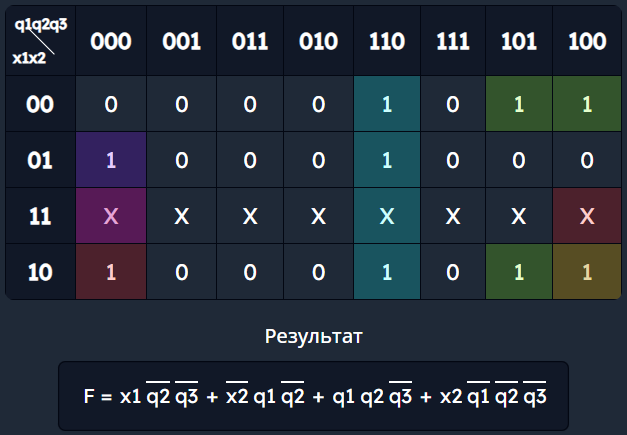
\includegraphics[width=0.9 \linewidth]{img/Q1.png}
	\caption{Минимизация для $Q_1$}
	\label{fig:Q1}
\end{figure}

\begin{figure}[H]
	\centering
	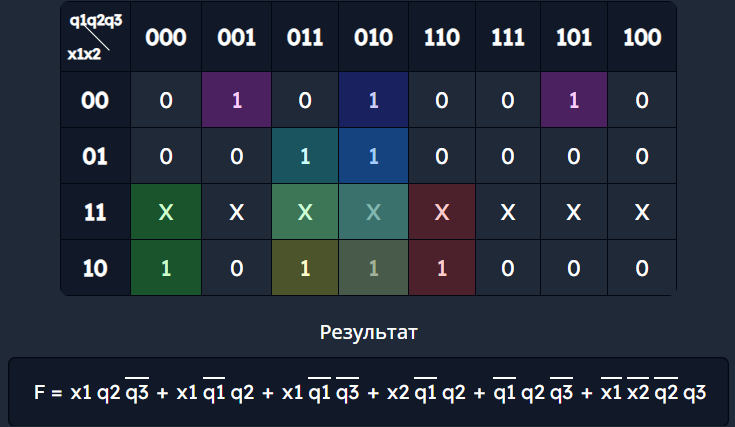
\includegraphics[width=0.9 \linewidth]{img/Q2.png}
	\caption{Минимизация для $Q_2$}
	\label{fig:Q2}
\end{figure}

\newpage
\begin{figure}[H]
	\centering
	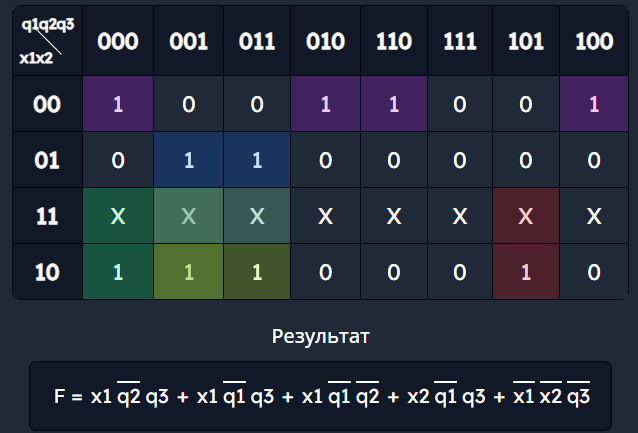
\includegraphics[width=0.9 \linewidth]{img/Q3.png}
	\caption{Минимизация для $Q_3$}
	\label{fig:Q3}
\end{figure}


\subsection{Минимизация для $\mathbf{L_1-L_6}$}

На \hyperref[fig:L1]{рисунках 5--10} приведены минимизации для потенциальный управляющих сигналов $L_1$--$L_6$ кодировки при помощи карт Карно.

\begin{figure}[ht]
	\centering
	\begin{minipage}{0.45\textwidth}
		\centering
		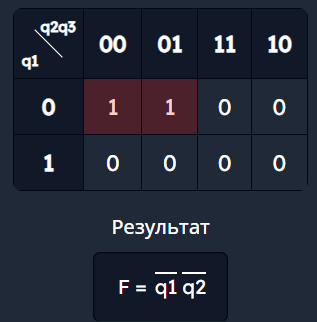
\includegraphics[width=\linewidth]{img/L1.png}
		\caption{Минимизация для $L_1$}
		\label{fig:L1}
	\end{minipage}\hfill
	\begin{minipage}{0.45\textwidth}
		\centering
		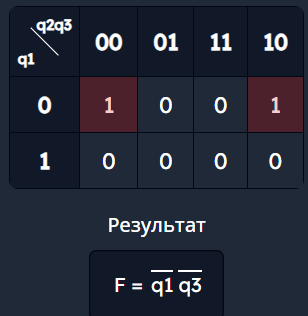
\includegraphics[width=\linewidth]{img/L2.png}
		\caption{Минимизация для $L_2$}
		\label{fig:L2}
	\end{minipage}
\end{figure}

\newpage

\begin{figure}[ht]
	\centering
	\begin{minipage}{0.45\textwidth}
		\centering
		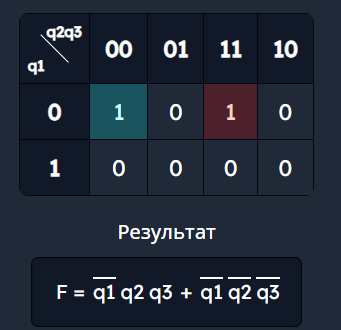
\includegraphics[width=\linewidth]{img/L3.png}
		\caption{Минимизация для $L_3$}
		\label{fig:L3}
	\end{minipage}\hfill
	\begin{minipage}{0.45\textwidth}
		\centering
		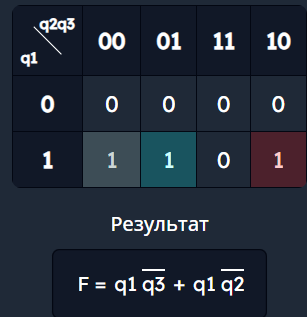
\includegraphics[width=\linewidth]{img/L4.png}
		\caption{Минимизация для $L_4$}
		\label{fig:L4}
	\end{minipage}
	
	\vspace{0.5cm}
	
	\begin{minipage}{0.45\textwidth}
		\centering
		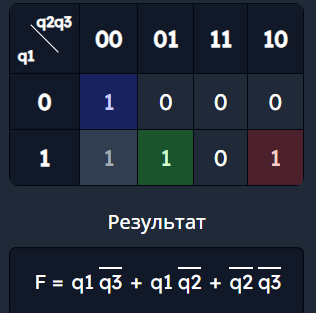
\includegraphics[width=\linewidth]{img/L5.png}
		\caption{Минимизация для $L_5$}
		\label{fig:L5}
	\end{minipage}\hfill
	\begin{minipage}{0.45\textwidth}
		\centering
		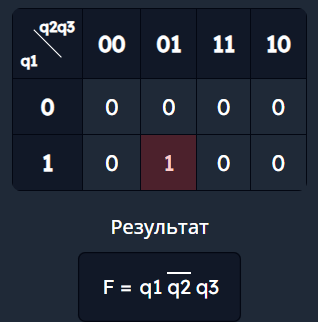
\includegraphics[width=\linewidth]{img/L6.png}
		\caption{Минимизация для $L_6$}
		\label{fig:L6}
	\end{minipage}
\end{figure}


\subsection{Минимизация для $\mathbf{i_1-i_4}$}

На \hyperref[fig:i1]{рисунках 11--14} представлены минимизации для импульсных управляющих сигналов $i_1$--$i_4$ кодировки при помощи карт Карно.

\newpage
\begin{figure}[H]
	\centering
	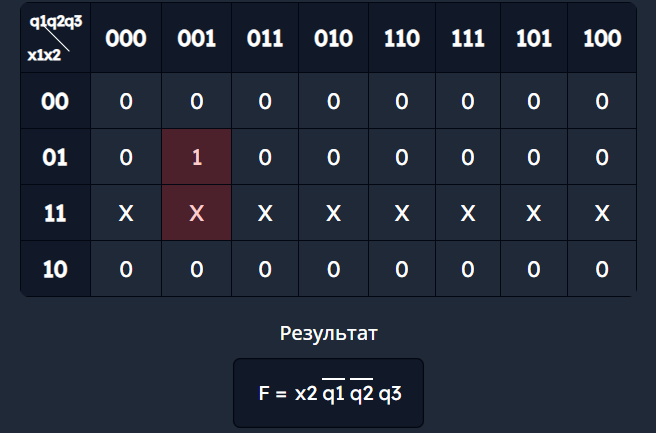
\includegraphics[width=0.9 \linewidth]{img/i1.png}
	\caption{Минимизация для $i_1$}
	\label{fig:i1}
\end{figure}

\begin{figure}[H]
	\centering
	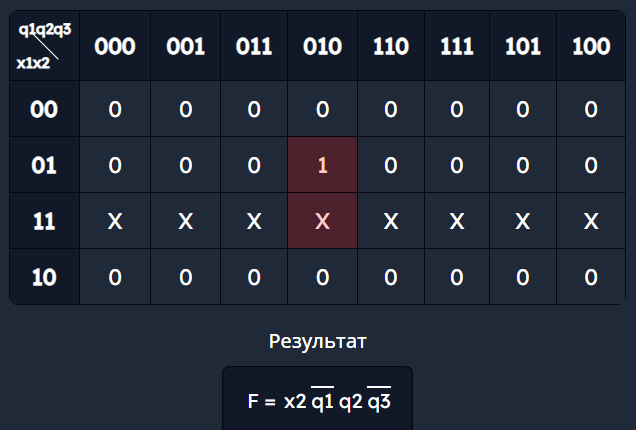
\includegraphics[width=0.9 \linewidth]{img/i2.png}
	\caption{Минимизация для $i_2$}
	\label{fig:i2}
\end{figure}

\newpage
\begin{figure}[H]
	\centering
	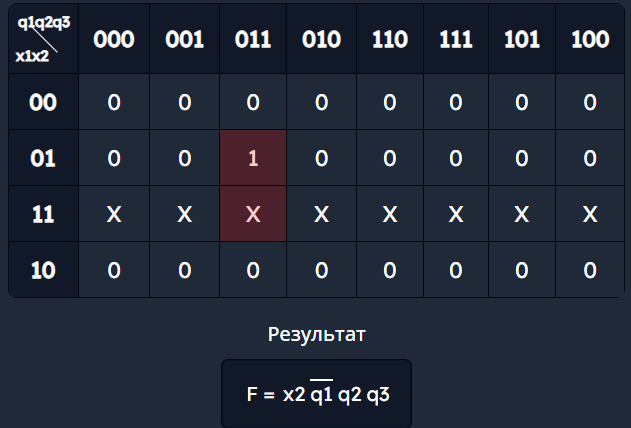
\includegraphics[width=0.9 \linewidth]{img/i3.png}
	\caption{Минимизация для $i_3$}
	\label{fig:i3}
\end{figure}

\begin{figure}[H]
	\centering
	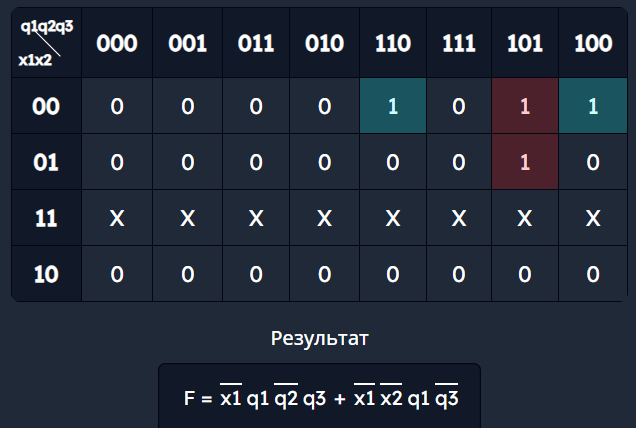
\includegraphics[width=0.9 \linewidth]{img/i4.png}
	\caption{Минимизация для $i_4$}
	\label{fig:i4}
\end{figure}

\newpage

\section{Схемотехническая реализация}

\subsection{Анализ схемотехнической реализации}

\subsubsection{Индикаторный преобразователь}

\textbf{Индикаторный преобразователь (ИП)} — это функциональная схема, предназначенная для преобразования числовой информации, представленной в двоичном коде, в сигналы, управляющие сегментами индикатора. В каждом разряде индикатор содержит семь сегментов, которые, высвечиваясь в определенной комбинации, могут дать изображение цифры. Для того, чтобы сегмент ''загорелся'', на него необходимо подать напряжение. Таким образом, один разряд индикатора содержит 7 входов. Если на некоторые из этих входов подать напряжение, а на остальные -- нет, то на индикаторе высветится соответствущая комбинация сегментов. Условное изображение схемы индикаторного преобразователя представлено на \hyperref[fig:IC1]{рисунке 15}, а его структурная схема на \hyperref[fig:IC2]{рисунке 16}.

\begin{figure}[ht]
	\centering
	\begin{minipage}{0.45\textwidth}
		\centering
		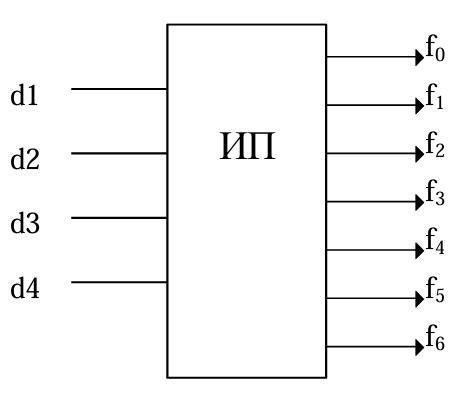
\includegraphics[width=\linewidth]{img/IC1.png}
		\caption{Схема ИП}
		\label{fig:IC1}
	\end{minipage}\hfill
	\hspace{0.5cm}
	\begin{minipage}{0.51\textwidth}
		\centering
		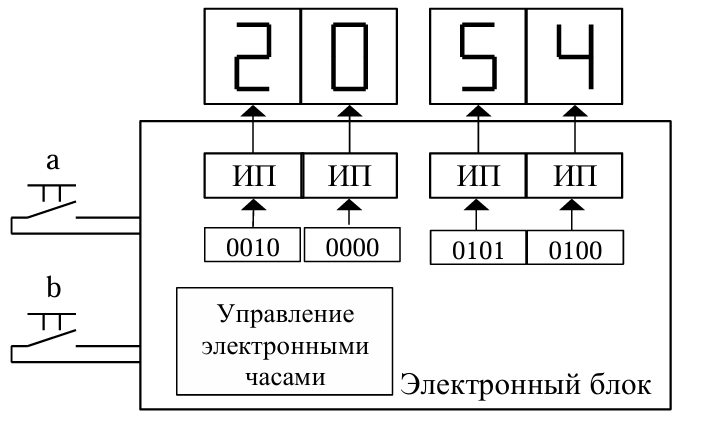
\includegraphics[width=\linewidth]{img/IC2.png}
		\caption{Структурная схема ИП}
		\label{fig:IC2}
	\end{minipage}
\end{figure}

В данной работе был создан ИП для отображения цифр от 0 до 9 включительно, его функциональная схема представлена на \hyperref[fig:IC]{рисунке 17.}

\newpage
\thispagestyle{empty}
\begin{figure}[H]
	\centering
	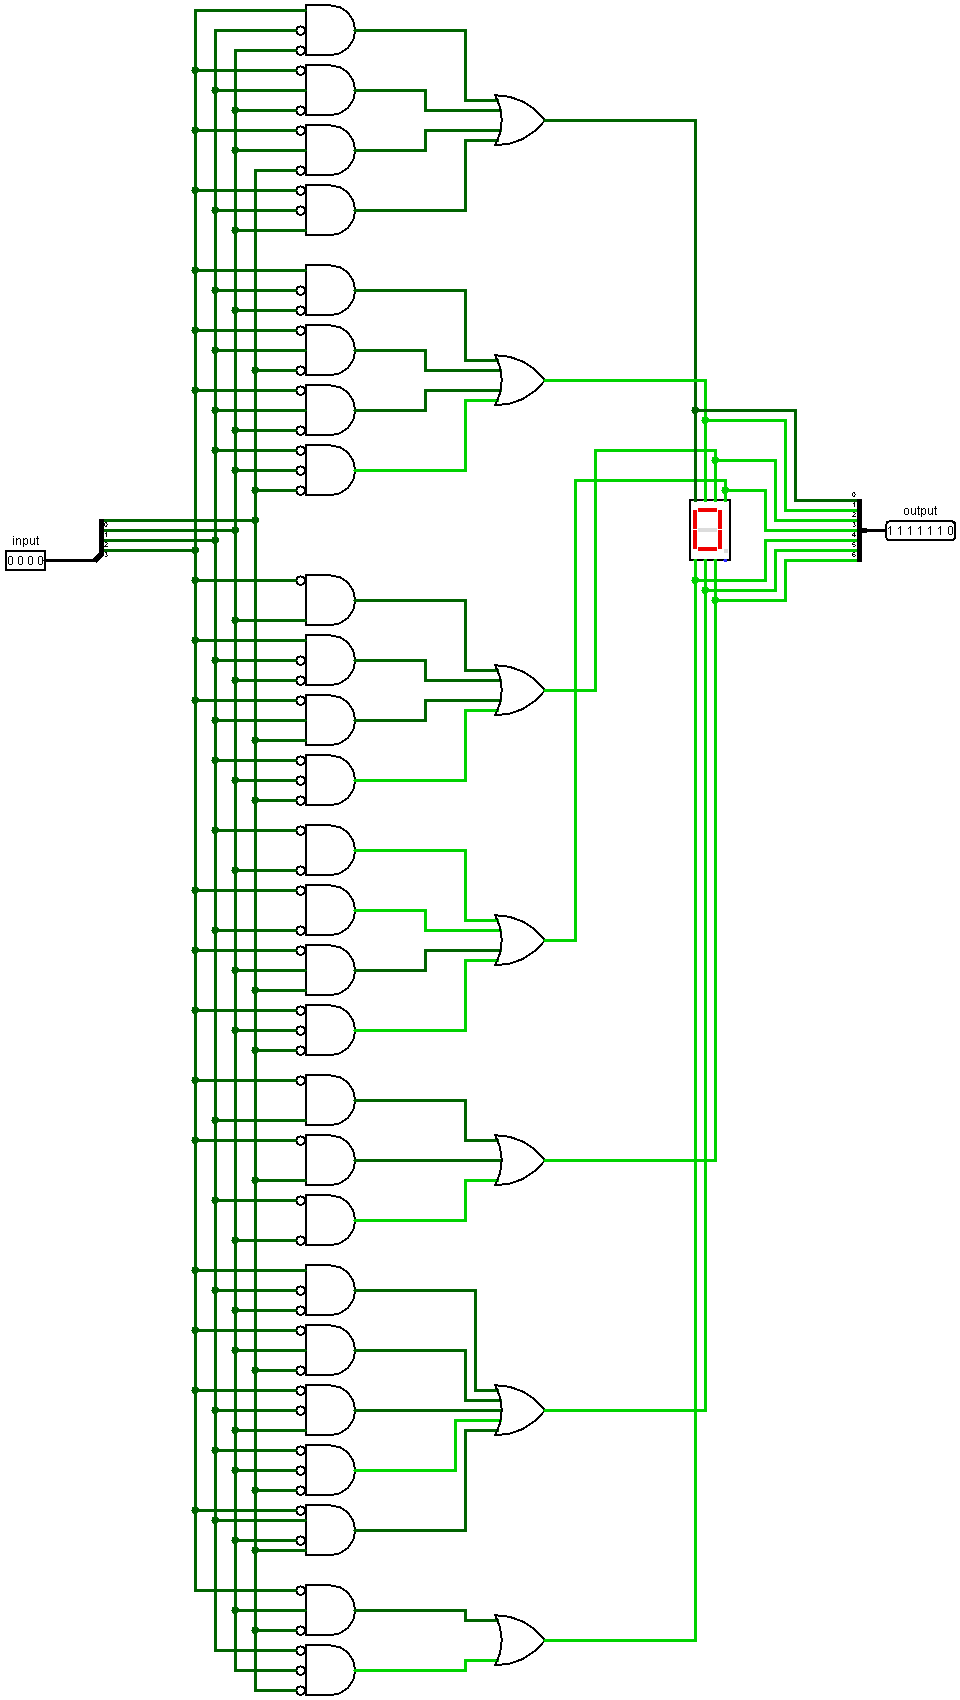
\includegraphics[width=0.85 \linewidth]{img/IC.png}
	\caption{Функциональная схема индикаторного преобразователя}
	\label{fig:IC}
\end{figure}

\newpage

\subsubsection{Счётчик}

\textbf{Счётчик} -- это устройство, которое осуществляет счет и хранение кода числа подсчитанных импульсов. У 
каждого счетчика есть тактовый вход, на который поступают электрические импульсы, и несколько 
выходов, с которых можно снимать двоичный код числа, находящийся в счетчике. С каждым новым 
входным импульсом этот код изменяется: он может увеличиваться на 1 (суммирующий счетчик), 
уменьшаться на 1 (вычитающий счетчик) или изменяться в соответствии с каким-либо другим правилом. 

Важным параметром счетчика является \textbf{коэффициент пересчета К}. К - это максимальное число импульсов, 
которое может быть подсчитано. Для удобства использования счетчика, кроме тактового входа существует вход 
“Уст.0” (сброс). При подаче на него импульса (логической единицы) на выходе устанавливается нулевой 
код. 


Функциональная схема счетчика с коэффициентом пересчёта К = 10, используемая в данной работе, представлена на 
\hyperref[fig:IC2]{рисунке 18}.

\begin{figure}[H]
	\centering
	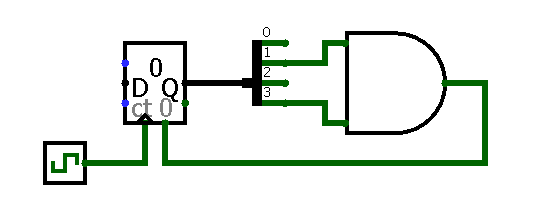
\includegraphics[width=0.68 \linewidth]{img/counter.png}
	\caption{Функциональная схема счётчика с К=10}
	\label{fig:counter}
\end{figure}


\subsubsection{Тактовый генератор}

\textbf{Генератор тактовых импульсов} — это компонент, который генерирует последовательную череду электрических сигналов (прямоугольных импульсов) с фиксированной частотой, используемых для синхронизации работы цифровых схем, таких как счётчики, триггеры и регистры. В данной работе, один такт генератора импульсов эквивалентен интервалу в одну секунду на часах, т.е. частоте 1 Гц. 

Функциональная схема тактового генератора, используемая в данной работе, представлена на \hyperref[fig:gen]{рисунке 19}.

\begin{figure}[H]
	\centering
	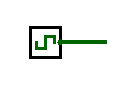
\includegraphics[width=0.25 \linewidth]{img/gen.png}
	\caption{Функциональная схема генератора тактовых импульсов}
	\label{fig:gen}
\end{figure}

\newpage

\subsubsection{Тоннель}

\textbf{Тоннель} -- это компонент, который используется для упрощения схем, сокращая длину проводников. Тоннель позволяет подключать элементы, расположенные на разных частях схемы, без необходимости протягивать длинные провода через весь рабочий участок. Он действует как виртуальная связь, передавая сигнал из одного места схемы в другое. Тоннель имеет только один контакт, разрядность которого соответствует атрибуту <<Биты данных>> тоннеля.

Функциональная схема тоннеля sec\_units, отвечающего за передачу сигнала, который представляет единицы секунд на часах и имеющего разрядность 4 бита представлена на \hyperref[fig:tunnel]{рисунке 20}.

\begin{figure}[H]
	\centering
	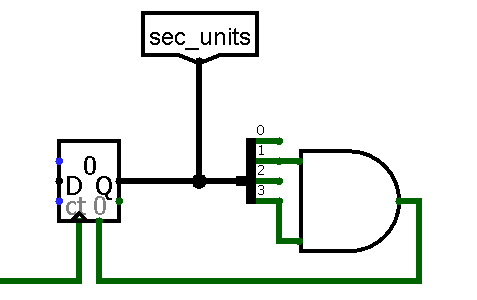
\includegraphics[width=0.55 \linewidth]{img/tunnel.png}
	\caption{Функциональная схема тоннеля}
	\label{fig:tunnel}
\end{figure}


\subsubsection{D-триггер}

Триггер -- это устройство с двумя устойчивыми состояниями. Основная его функция -- хранить один бит информации неограниченное время до тех пор, пока эта информация не будет изменена воздействием на вход триггера. Существует довольно много разновидностей триггеров, различающихся по входным условиям смены состояния. 
 
В данной работе используется D-триггер, представленный на \hyperref[fig:trigger]{рисунке 21}. D-триггер (или D-Flip-Flop) — это базовый элемент памяти, который сохраняет значение, поданное на его вход \textbf{D}, на выходе \textbf{Q} до следующего тактового сигнала. 

D-триггер имеет несколько ключевых входов:
\begin{itemize}
	\item \textbf{D} — вход данных, на который подается значение, которое будет сохранено в триггере.
	\item \textbf{Clock (C)} — тактовый сигнал, который управляет моментом записи данных на выход. Запись происходит на фронте тактового сигнала (обычно на переднем фронте).
	\item \textbf{Q} — основной выход, на котором сохраняется информация, поступившая на вход \textbf{D}.
	\item \textbf{Q'} — инвертированный выход, который является логическим дополнением выхода \textbf{Q}.
\end{itemize}
 
D-триггер сохраняет значение на выходе \textbf{Q} до тех пор, пока не будет активирован тактовый сигнал. Когда тактовый сигнал меняет свое состояние (например, с 0 на 1), информация с входа \textbf{D} копируется в триггер и сохраняется на выходе \textbf{Q}. Это значение будет сохраняться до следующего тактового импульса.

\begin{figure}[H]
	\centering
	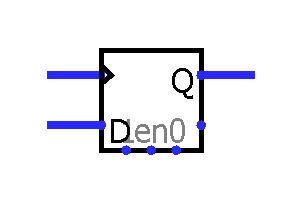
\includegraphics[width=0.35 \linewidth]{img/trigger.png}
	\caption{Функциональная схема триггера}
	\label{fig:trigger}
\end{figure}


\subsubsection{Преобразователь внешних воздействий}

Функциональная схема преобразователя внешних воздействий (\hyperref[fig:influence]{рис. 22}) предназначена для преобразования сигналов, поступающих с кнопок, в закодированные сигналы. Она реализует функциональность конечного автомата, где на основе нажатия кнопок формируются выходные сигналы в виде кодов 00, 01 или 10. Кроме того, в схеме используется синхроимпульс — импульс, поступающий от кнопки, который синхронизирует обновление состояния конечного автомата. Этот импульс подается на вход \textbf{Clock} D-триггера, что заставляет триггер запомнить текущее состояние.

\begin{figure}[H]
	\centering
	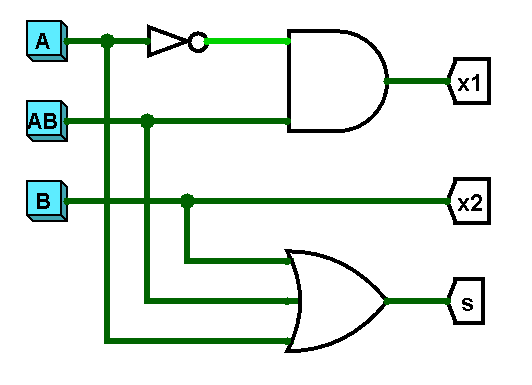
\includegraphics[width=0.45 \linewidth]{img/input-converter.png}
	\caption{Функциональная схема преобразователя внешних воздействий}
	\label{fig:influence}
\end{figure}


\subsubsection{Блок элементов памяти}

Блок элементов памяти представляет собой ряд D-триггеров, которые отвечают за хранение текущего состояния автомата. Каждый D-триггер сохраняет один бит информации, необходимой для представления состояния системы. 

Работа этого блока синхронизируется с помощью \textbf{синхроимпульса} — тактового сигнала, который подается на вход \textbf{Clock} каждого триггера. Синхроимпульс определяет момент времени, когда данные, поступающие на входы триггеров, записываются в их внутреннюю память. Это позволяет всей системе обновлять свое состояние строго в согласованные моменты времени, исключая возможные ошибки или несоответствия между состояниями отдельных триггеров.

Синхроимпульс формируется генерируется внутри схемы в ответ на нажатие кнопки. При поступлении синхроимпульса все триггеры одновременно фиксируют свои входные значения на выходах, сохраняя новое состояние автомата. Функциональная схема блока элементов памяти в составе i-формирователя (\hyperref[sec:i]{см. раздел i-формирователя}) представлена на \hyperref[fig:icov]{рисунке 23}.

\begin{figure}[H]
	\centering
	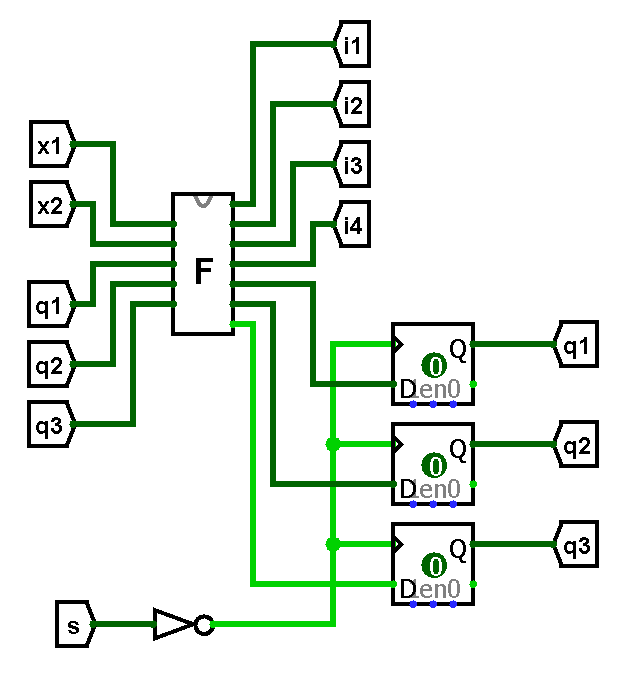
\includegraphics[width=0.65 \linewidth]{img/i-converter.png}
	\caption{Функциональная схема i-формирователя с блоком элементов памяти}
	\label{fig:icov}
\end{figure}


\subsubsection{Блок F}

Блок F отвечает за вычисление следующего состояния конечного автомата, а также вычисляет, требуется ли по текущему входу и текущему состоянию формировать импульсный сигнал. Сам блок представляет из себя множество логических блоков, рассматривающих каждую ситуацию изменения состояния конечного автомата и формирования импульсного сигнала. Блок F представлен на \hyperref[fig:F]{рисунке 24}.

\begin{figure}[H]
	\centering
	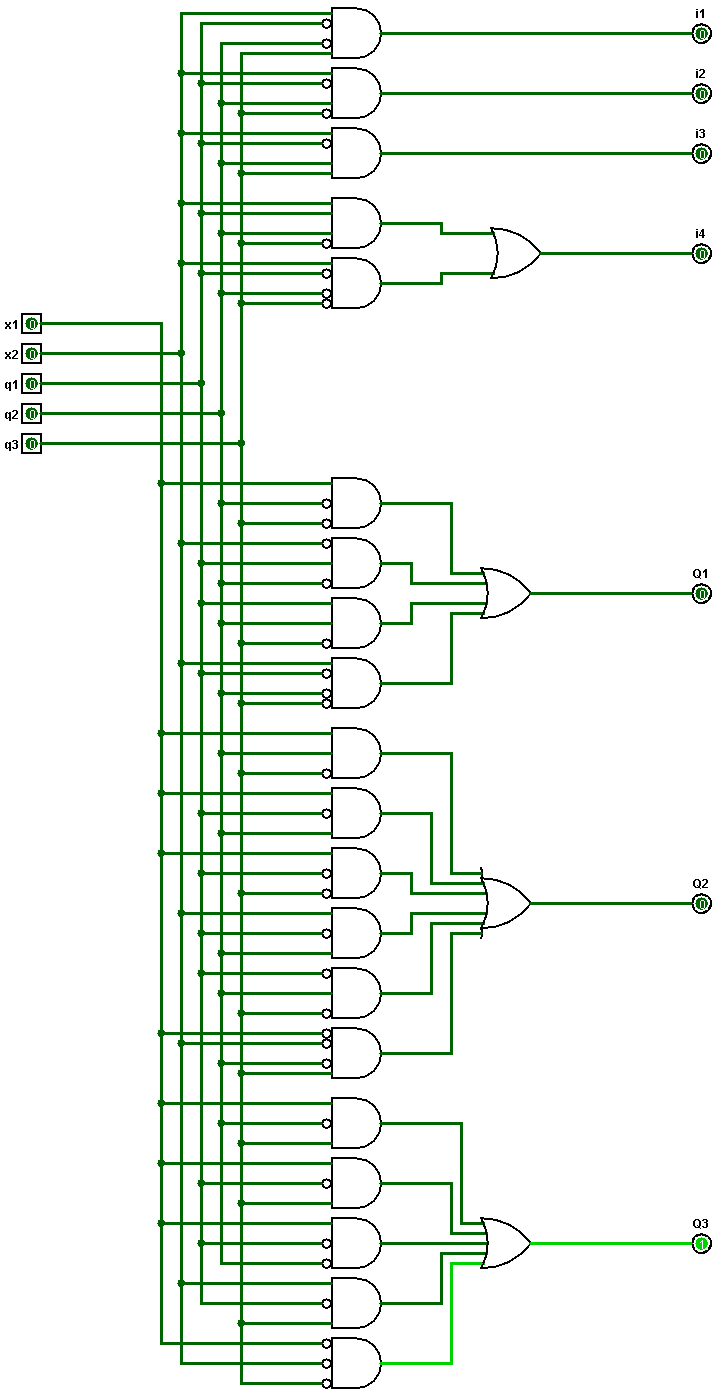
\includegraphics[width=0.75 \linewidth]{img/F.png}
	\caption{Функциональная схема блока F}
	\label{fig:F}
\end{figure}

\subsubsection{Блок FL}
Блок F отвечает за формирование потенциальных сигналов, относительно текущего состояния автомата. Он также как и блок F представляет из себя множество логических блоков, которые рассматривают ситуации формирования потенциального сигнала относительно текущего состояния автомата. Функциональная схема блока FL представлена на \hyperref[fig:FL]{рисунке 25}.

\begin{figure}[H]
	\centering
	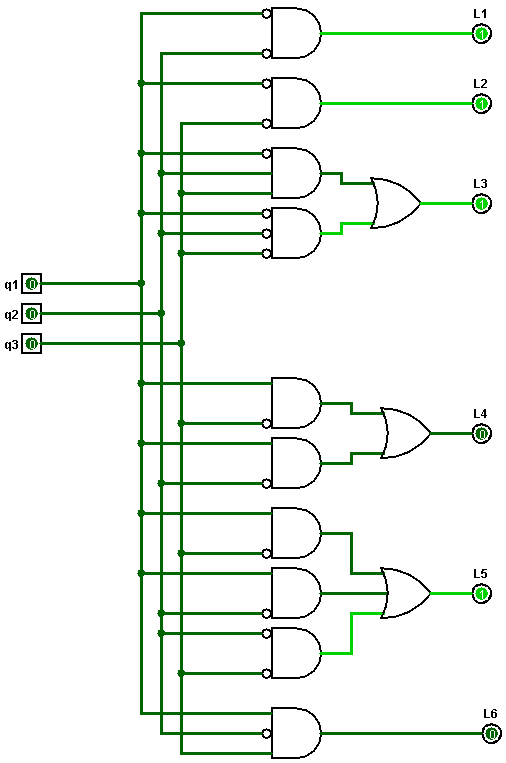
\includegraphics[width=0.75 \linewidth]{img/FL.png}
	\caption{Функциональная схема блока FL}
	\label{fig:FL}
\end{figure}

\subsubsection{i-формирователь}
\label{sec:i}

i-формирователь отвечает за генерацию импульсного сигнала. Он получает на вход продолжительный сигнал от блока F. Когда на i-формирователь подаётся синхроинпульс, он генерирует импульсный сигнал. Функциональная схема i-формирователя представлена на \hyperref[fig:icov]{рисунке 26}.

\begin{figure}[H]
	\centering
	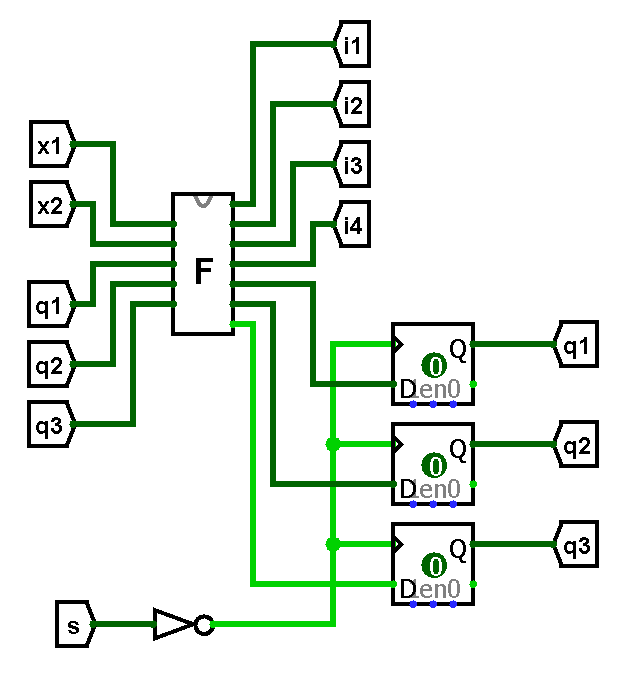
\includegraphics[width=0.65 \linewidth]{img/i-converter.png}
	\caption{Функциональная схема i-формирователя}
	\label{fig:icov}
\end{figure}


\subsubsection{Интерфейс часов}

Интерфейс часов включает в себя 5 дисплеев. Назначение дисплеев слева направо: отображение старшего разряда числа часов, отображение младшего разряда числа часов, отображение старшего разряда числа минут, отображения младшего разряда числа минут, отображение a.m./p.m. Также состояния включен/выключен у дисплеев регулируются потенциальными сигналами $L_1$, $L_2$, $L_3$, $L_4$. Когда происходит корректировка времени или установка времени будильника, то включены только те дисплеи, изменение времени на которых происходит в данный момент, когда как остальные дисплеи отключены. Эта логика достигается благодаря переключателям, которые перестают пропускать ток, когда на них самих нет тока. Интерфейс часов представлен на \hyperref[fig:watch]{рисунке 27}.


\begin{figure}[H]
	\centering
	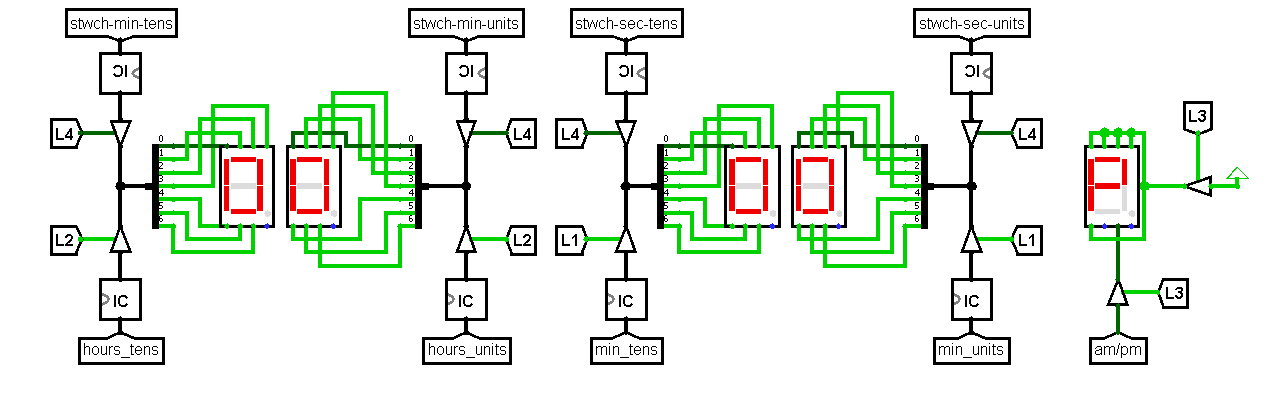
\includegraphics[width=1.0 \linewidth]{img/watch.png}
	\caption{Функциональная схема реализации интерфейса часов}
	\label{fig:watch}
\end{figure}


\subsubsection{Секундомер}
Секундомер представляет из себя подсхему часов. Он обладает 4-я счётчиками, двумя для хранения цифр минут в старшем и младшем разряде, и ещё двумя для хранения цифр секунд в старшем и младшем разряде. Функциональная схема секундомера представлена на \hyperref[fig:stopwatch]{рисунке 28}.

\begin{figure}[H]
	\centering
	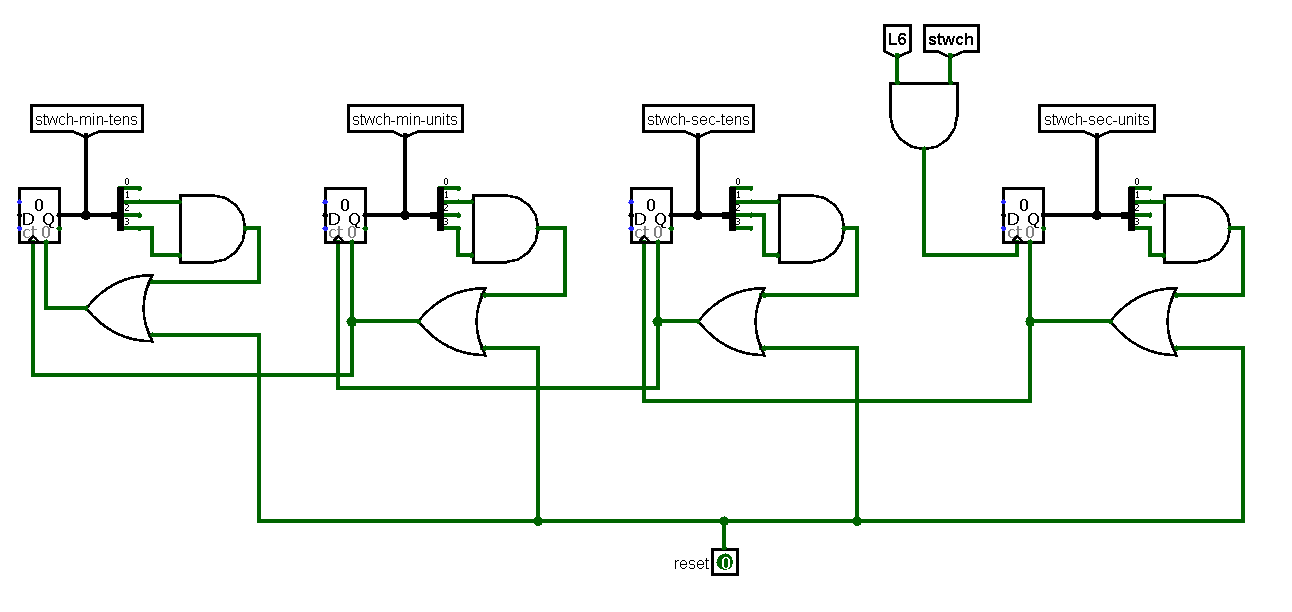
\includegraphics[width=1.0 \linewidth]{img/stopwatch.png}
	\caption{Функциональная схема секундомера}
	\label{fig:stopwatch}
\end{figure}

\subsection{Расчёт площади схемы}

Количество компонентов каждого типа на функциональной схеме часов показано на \hyperref[fig:stats]{рисунке 29}.

\newpage
\begin{figure}[H]
	\centering
	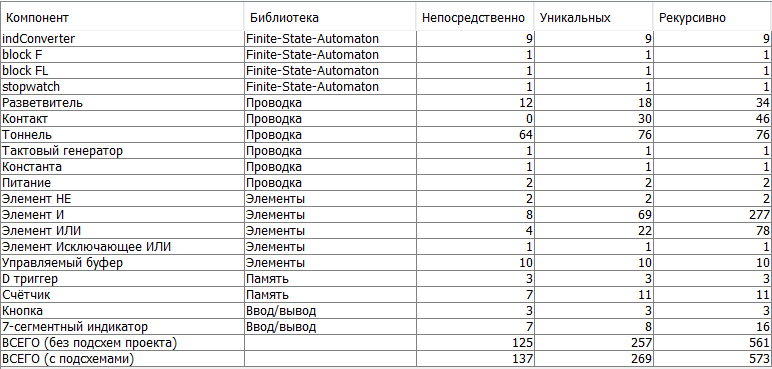
\includegraphics[width=1.0 \linewidth]{img/stats.png}
	\caption{Статистика функциональной схемы часов}
	\label{fig:stats}
\end{figure}

Рассчитаем число транзисторов для каждого компонента с учётом количества его вхождений в схему(рекурсивно). Результат представлен в 

\begin{table}[H]
	\centering
	\caption*{Рис. 37. Подсчёт количества транзисторов на функциональной схеме.}
	\small{
		\begin{tabular}{|c|c|c|c|}
			\hline
			Элемент & Число транзисторов & Число элементов & Всего транзисторов  \\ 
			\hline
			Элемент И & 4 & 277 & 1108  \\ 
			\hline
			Элемент НЕ & 4 & 2 & 8  \\ 
			\hline
			Элемент ИЛИ & 6 & 78 & 468  \\ 
			\hline
			Элемент XOR & 10 & 1 & 10  \\ 
			\hline
			D-триггер & 20 & 3 & 60  \\ 
			\hline
			Счётчик 4-разрядный & 64 & 10 & 640 \\ 
			\hline
			Счётчик 1-разрядный & 16 & 1 & 16 \\ 
			\hline
			Индикаторный преобразователь & 400 & 9 & 3600 \\ 
			\hline
		\end{tabular}
	}
\end{table}

Просуммировав последний столбец таблицы можно получить, что на всю функциональную схему приходится \textbf{5910}. Исходя из расчёта, что на 1 квадратный миллиметр приходится примерно 1000 транзисторов, функциональная схема реализованных часов должна занимать примерно \textbf{5.910 ${\text{мм}}^2$}.


\newpage
\section*{Заключение}
\addcontentsline{toc}{section}{Заключение}
В ходе выполнения курсовой работы была разработана функциональная схема часов, реализующих следующие функции:
\begin{itemize}
	\item \textbf{Отображение и корректировка минут, часов:} Часы позволяют отображать текущее время на индикаторах, разделённое на минуты и часы. Корректировка осуществляется с помощью кнопок ''a'', ''b'', которые позволяют по отдельности изменять значение минут и часов.
	\item \textbf{12-и часовой формат времени:} Временной формат ограничен диапазоном от 12:00 AM до 11:59 PM. При достижении значения 12 часов выполняется переход между AM (до полудня) и PM (после полудня), что отражается на индикаторах.
	\item \textbf{Простой секундомер (сброс-запуск-остановка):} Секундомер запускается нажатием кнопки ''a'' и начинает отсчёт времени в секундах. Максимальное значение на секундомере -- 99 минут, 99 секунд. Остановка осуществляется кнопкой ''a'', а сброс выполняется при нажатии на кнопку ''b'', как во время работающего секундомера, так и при паузе.
	\item \textbf{Остановка часов по нажатию кнопки:} Предусмотрена возможность приостановки работы часов при нажатии на кнопку ''ab'': текущее время замораживается на экране, и отсчёт секунд, минут и часов временно прекращается. Возобновление работы выполняется нажатием любой другой кнопки.
\end{itemize}
Преимущества реализованной функциональной схемы часов:
\begin{itemize}
	\item При минимизации функций блоков FL, F и i-формирователя использовалась недоопределённость частичных функций.
	\item Наличие отключения/включения дисплеев во время корректировки времени.
\end{itemize}
Недостатки реализованной функциональной схемы часов:
\begin{itemize}
	\item Избыточное состояние ''пауза'' в конечном автомате. Вместо него, можно было бы останавливать секундомер при нажатии на кнопку ''ab'', находясь в состоянии ''reset stopwatch'', и возобновлять работу секундомера при переходе в состояние ''running stopwatch''. 
\end{itemize}
Также у данной схемы имеется некоторый задел на масштабирование:
\begin{itemize}
	\item Реализация звукового сигнала каждое через каждое n-ое количество минут.
	\item Добавить дисплей для отображения секунд.
	\item Отключение индикаторов с целью экономии энергии.
	\item Добавление будильника в функционал часов.
\end{itemize}


\newpage
\addcontentsline{toc}{section}{Список использованной литературы}
\begin{thebibliography}{0}
	\bibitem{tema} Методические указания к курсовой работе [Электронный ресурс]. Сайт секции «Телематика». — URL: \href{https://tema.spbstu.ru/userfiles/files/courses/2018-theory-algorithm/KuR_MU.pdf}{https://tema.spbstu.ru/userfiles/files/courses/2018-theory-algorithm/KuR\_MU.pdf} (дата обращения: 08.01.2025).
	\bibitem{karpov}  Карпов Ю.Г. Теория автоматов. - СПб.: Питер, 2003. - 224 с.
	\bibitem{Ericson} Эриксон Д. Алгоритмы. - М.: ДМК-Пресс, 2023. - 526 с.
	\bibitem{site} Карта Карно [Электронный ресурс]. — URL: \href{https://sublime.tools/ru/karta-karno}{https://sublime.tools/ru/karta-karno} (дата обращения: 12.01.2025).
	
\end{thebibliography}

\addcontentsline{toc}{section}{Приложение. Общая функциональная схема часов}
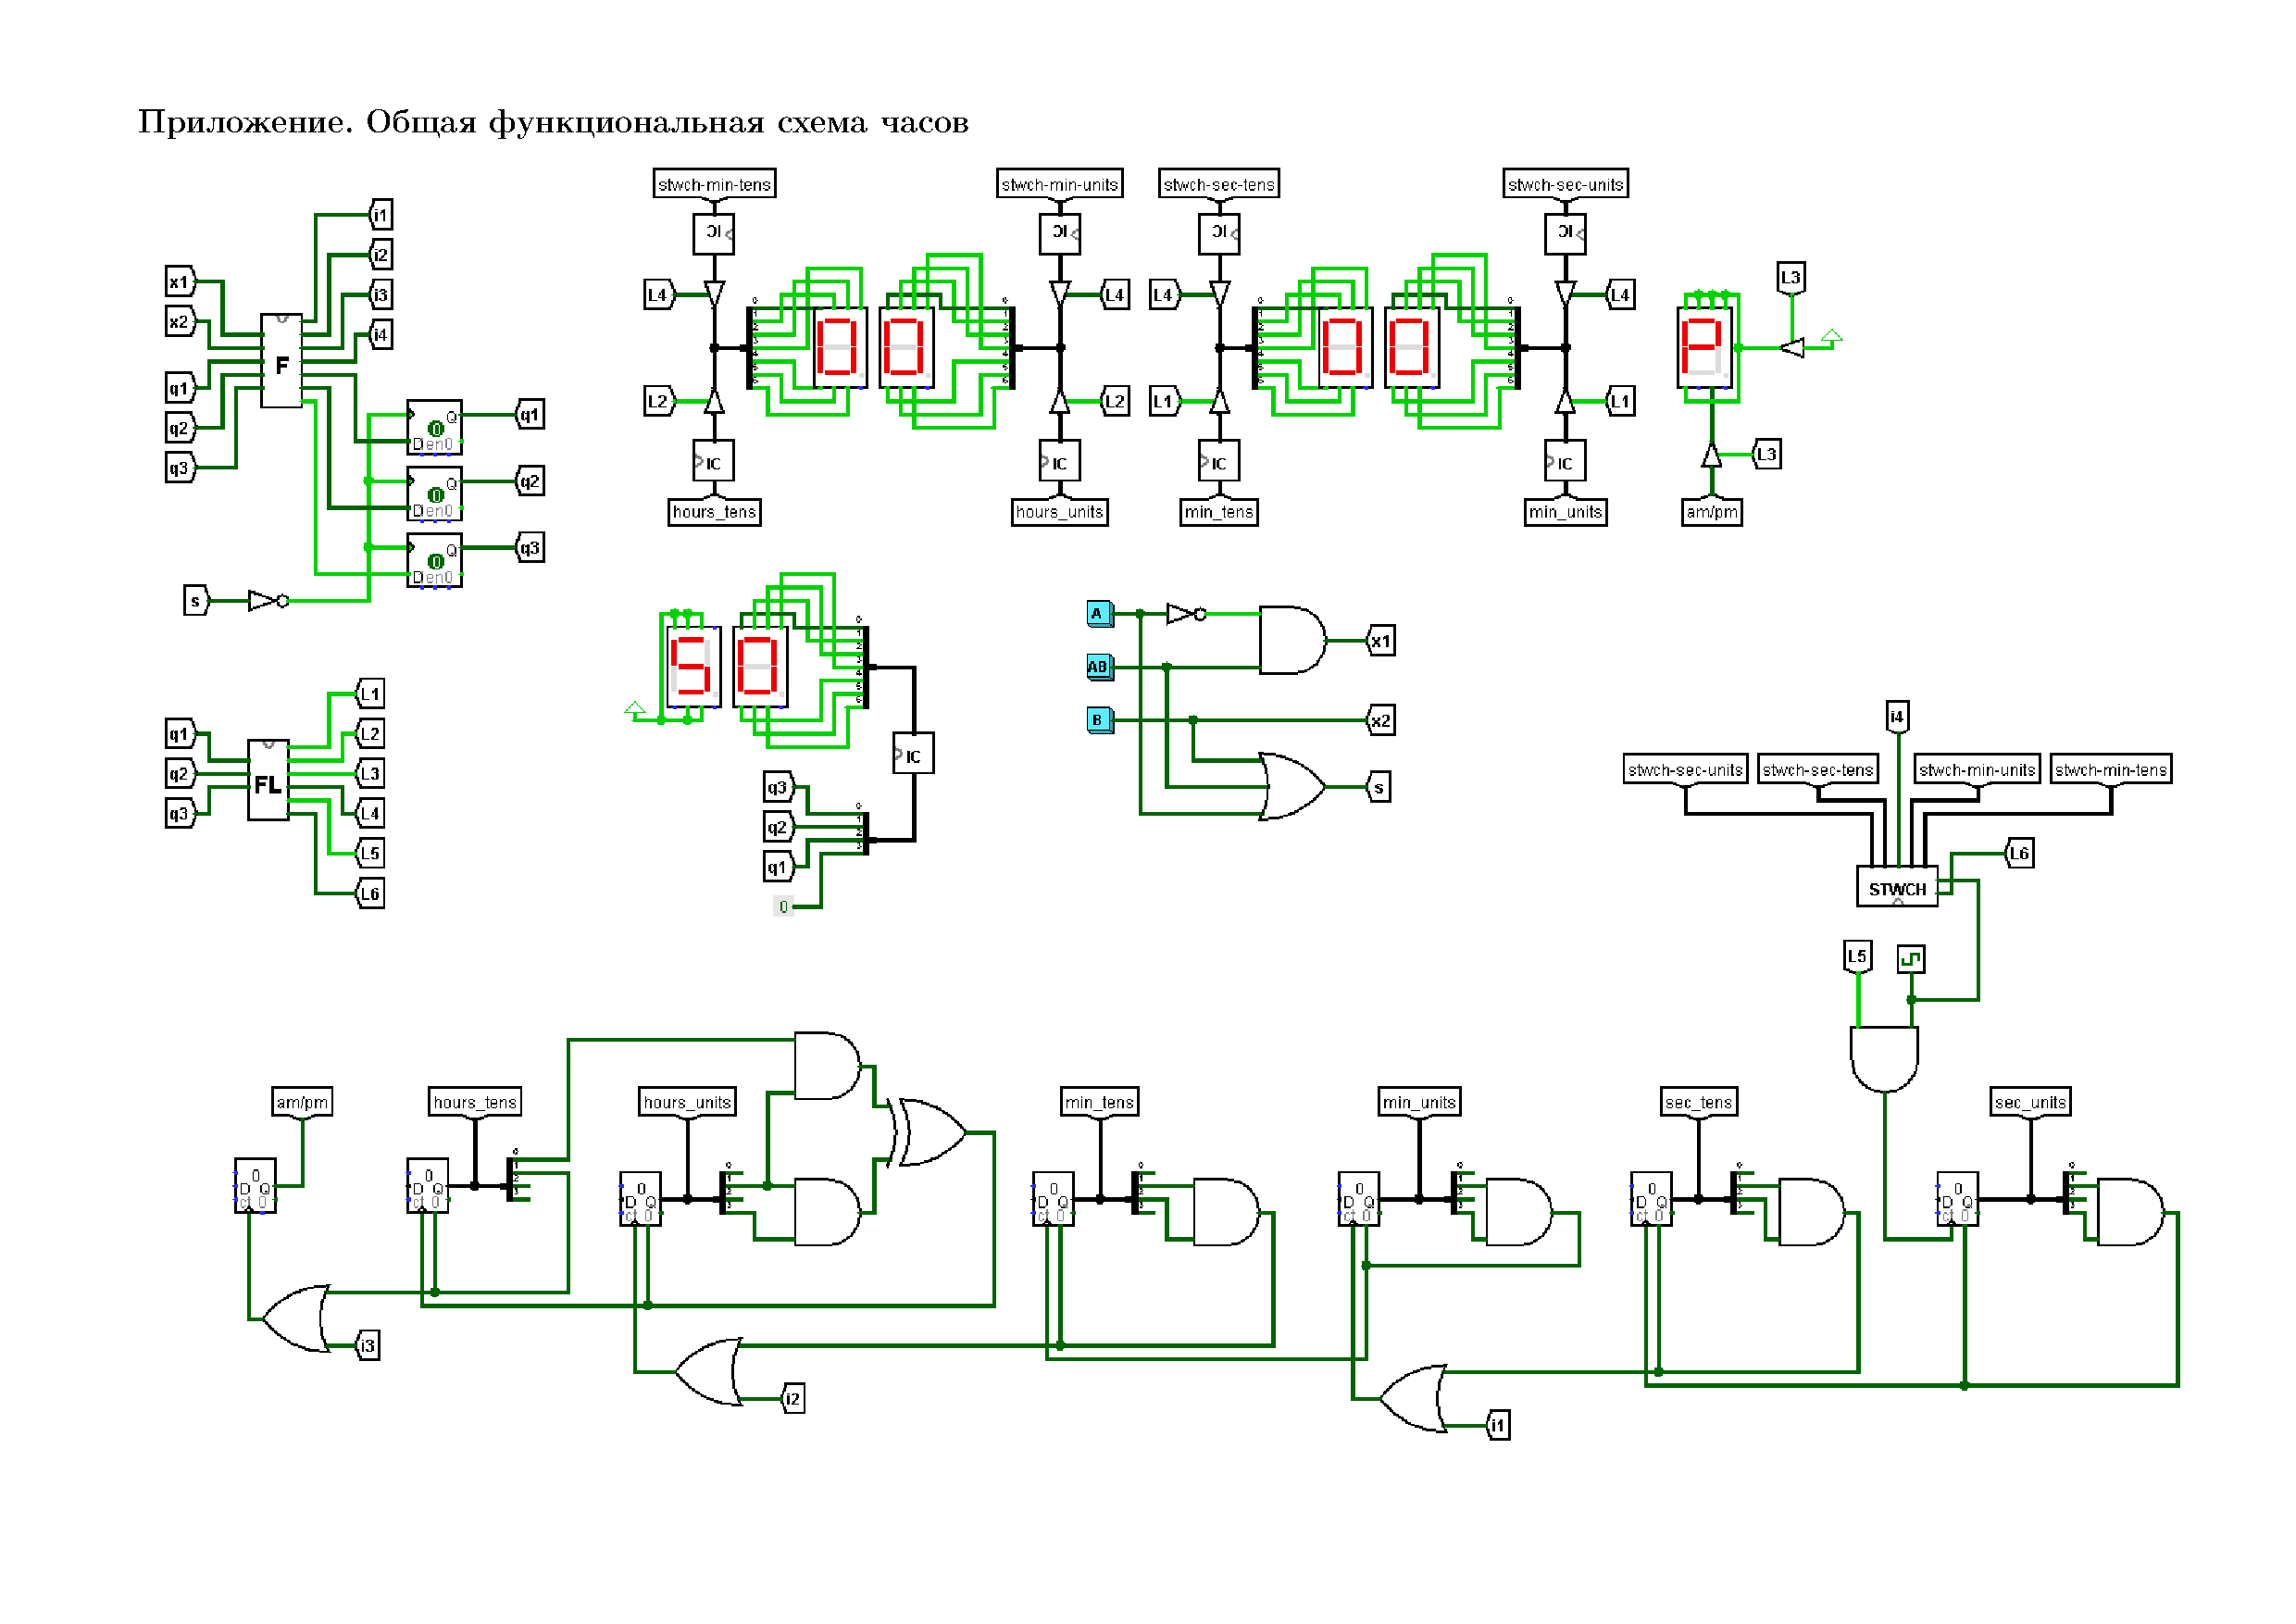
\includepdf[pages=-,fitpaper]{scheme.pdf} 



\end{document}